
%%%%%%%%%%%%%%%%%%%%%%%%%%%%%%%%%%%%%%%%%%%%%%%%%%%%%%%%%%%%%%%%%%%%%%%%%%%%%%%%%%%%%%%
%%%%%%%%%%%%%%%%%%%%%%%%%%%%%%%%%%%%%%%%%%%%%%%%%%%%%%%%%%%%%%%%%%%%%%%%%%%%%%%%%%%%%%%
%%%%%%%%%%%%%%%%%%%%%%%%%%%%%%%%%%%%%%%%%%%%%%%%%%%%%%%%%%%%%%%%%%%%%%%%%%%%%%%%%%%%%%%
\section{Serie de Taylor de $f(x)$, $e(\VECTOR{x})$ e $\VECTOR{f}(\VECTOR{x})$}
\label{def:taylor}


\index{Serie de Taylor!$f:\mathbb{R} \rightarrow \mathbb{R}$}
\begin{proposition}[Serie de Taylor de $d(x)$:]\label{prop:taylord}
Dada uma função $f:\mathbb{R}\rightarrow \mathbb{R}$ com variável $x \in \mathbb{R}$;
infinitamente diferenciável em $a \in \mathbb{R}$;
esta pode ser expressada mediante uma somatória, em serie de Taylor 
\cite[pp. 734]{stewart2008calculus} \cite[pp. 281]{telles2015matematica} \cite{Taylor} 
ao redor de $a$, como
mostra a Eq. (\ref{eq:taylord1}),% onde $\left.\frac{\partial^k f(x)}{\partial x^k}\right|_{x=a}\equiv f^{(k)}(a) $.
\begin{equation}\label{eq:taylord0a}
\left.\frac{\partial^k f(x)}{\partial x^k}\right|_{x=a}\equiv f^{(k)}(a) 
\end{equation}
\begin{equation}\label{eq:taylord1}
  f(x)=f(a)
      ~+\frac{f'(a)}{1!} (x-a)
      ~+\frac{f''(a)}{2!} (x-a)^{2}
      ~+\cdots 
      ~+\frac{f^{(k)}(a)}{k!} (x-a)^{k}
      ~+\cdots 
\end{equation}
A equação pode ser escrita de forma mais compacta mediante uma somatória  como mostra a Eq. (\ref{eq:taylord2}),
\begin{equation}\label{eq:taylord2}
  f(x)=\sum\limits_{k=0}^{+\infty} \frac{f^{(k)}(a)}{k!} (x-a)^{k}.
\end{equation}
\end{proposition}

\begin{proposition}[Polinômio de Taylor com resto $R_n(x)$ de Lagrange:]\label{prop:polytaylor}
Dada uma função $f:\mathbb{R}\rightarrow \mathbb{R}$ com variável $x \in \mathbb{R}$;
esta pode ser expressada mediante uma somatória finita, $f_n(x)$, 
em polinômio de Taylor de grau $n$ ao redor de $a$
\cite[pp. 737]{stewart2008calculus} \cite[pp. 285]{telles2015matematica}, 
 como mostra a Eq. (\ref{eq:polytaylord1}),
\begin{equation}\label{eq:polytaylord1}
  f_n(x)=\sum\limits_{k=0}^{n} \frac{f^{(k)}(a)}{k!} (x-a)^{k},
\qquad
R_n(x)=\frac{f^{(n+1)}(z)}{(n+1)!} (x-a)^{n+1},
\end{equation}
\begin{equation}\label{eq:polytaylord2}
f(x)= f_n(x) + R_n(x);
\end{equation}
onde $z \in ]a,x[$, quando $x>a$, e $z \in ]x,a[$, quando $x<a$.
\end{proposition}


\begin{example}[Polinômio de Taylor do $cos(x)$:]
Aproximar a função $f(x)=cos(x)$ usando o polinômio de Taylor ao redor do ponto $a=0$,
numa versão truncada ate a derivada de ordem $4$, $8$ e $10$,
denominados aqui $f_4(x)$, $f_8(x)$ e $f_{10}(x)$, respetivamente.
\end{example}
\begin{SolutionT}[Serie de Taylor do $cos(x)$:]
Usando a Proposição \ref{prop:taylord} é calculado $f^{(k)}(x)$ para os 10 primeiros termos,
\begin{equation}
f^{(k)}(x)=
\left\{
\begin{matrix}
cos(x) & ~if & (k~mod~4)=0\\
-sin(x)& ~if & (k~mod~4)=1\\
-cos(x)& ~if & (k~mod~4)=2\\
sin(x) & ~if & (k~mod~4)=3
\end{matrix}
\right.
\quad \rightarrow \quad
f^{(k)}(0)=
\left\{
\begin{matrix}
1 & ~if & (k~mod~4)=0\\
0& ~if & (k~mod~4)=1\\
-1& ~if & (k~mod~4)=2\\
0 & ~if & (k~mod~4)=3
\end{matrix}
\right.
\end{equation}

\begin{equation}
f_{4}(x)=
1
-\frac{x^{2}}{2!} 
+\frac{x^{4}}{4!},
\qquad 
f_{8}(x)=
1
-\frac{x^{2}}{2!} 
+\frac{x^{4}}{4!} 
-\frac{x^{6}}{6!} 
+\frac{x^{8}}{8!}, 
\end{equation}
\begin{equation}
f_{10}(x)=
1
-\frac{x^{2}}{2!} 
+\frac{x^{4}}{4!} 
-\frac{x^{6}}{6!} 
+\frac{x^{8}}{8!} 
-\frac{x^{10}}{10!} 
\end{equation}
As aproximações podem ser vistas graficamente na Fig. \ref{fig:taylore}.
\end{SolutionT}

\begin{figure}[!h]
  \centering
    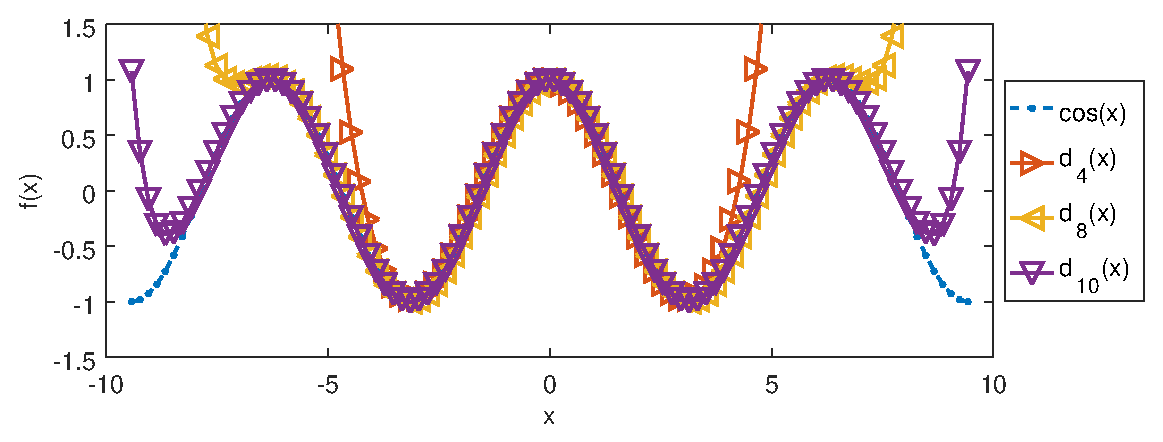
\includegraphics[width=0.90\textwidth]{chapters/funcoes/mcode/taylorR1R1/taylore.eps}
  \caption{Aproximação da função $cos(x)$ usando a serie de Taylor truncada.}
    \label{fig:taylore}
\end{figure}
 
%%%%%%%%%%%%%%%%%%%%%%%%%%%%%%%%%%%%%%%%%%%%%%%%%%%%%%%%%%%%%%%%%%%%%%%%%%%%%%%%%%%%%%%
 \index{Serie de Taylor!$f:\mathbb{R}^{N}\rightarrow \mathbb{R}$}
\begin{proposition}[Serie de Taylor de $f(\VECTOR{x})$]\label{prop:taylore}
Dada uma função $f:\mathbb{R}^{N}\rightarrow \mathbb{R}$ com variável $\VECTOR{x} \in \mathbb{R}^{N}$, vetor coluna;
infinitamente diferenciável em $\VECTOR{a} \in \mathbb{R}^{N}$;
esta pode ser expressada mediante uma somatória, em serie de Taylor 
\cite[pp. 187, 207]{zhang2017matrix} \cite{Taylor}  ao redor de $\VECTOR{a}$, como
mostra a Eq. (\ref{eq:taylore1}),
\begin{equation}\label{eq:taylore1}
f(\VECTOR{x}) =\sum _{k_{1}=0}^{\infty }\cdots \sum _{k_{N}=0}^{\infty }\left.\left({\frac {\partial ^{k_{1}+\cdots +k_{N}}f(\VECTOR{x})}{\partial x_{1}^{k_{1}}\cdots \partial x_{N}^{k_{N}}}}\right)\right|_{\VECTOR{x}=\VECTOR{a}} {\frac {(x_{1}-a_{1})^{k_{1}}\cdots (x_{N}-a_{N})^{k_{N}}}{k_{1}!\cdots k_{N}!}}
\end{equation}

Outra forma alternativa de expressar a função anterior é usando vetores e matrizes,
como na Eq. (\ref{eq:taylore2}).
\begin{equation}\label{eq:taylore2}
  f(\VECTOR{x})=f(\VECTOR{a})
      ~+ \triangledown f(\VECTOR{a})^{\transpose} (\VECTOR{x}-\VECTOR{a})
      ~+\frac{1}{2!}(\VECTOR{x}-\VECTOR{a})^{\transpose} \MATRIX{H(\VECTOR{a})}  (\VECTOR{x}-\VECTOR{a})
      ~+\cdots 
\end{equation}
Onde o vector $\triangledown f(\VECTOR{x})\equiv \frac{\partial f(\VECTOR{x})}{\partial \VECTOR{x} }$ 
(também chamado \hyperref[def:gradient]{gradiente}),
e a matriz $\MATRIX{H}(\VECTOR{x})\equiv \frac{\partial }{\partial \VECTOR{x}} \left( \frac{\partial f(\VECTOR{x})}{ \partial \VECTOR{x}^{\transpose} }\right)$
(também chamada matriz \hyperref[def:hessian]{Hessiana}).
\end{proposition}

\begin{example}[Serie de Taylor do 
$f(\VECTOR{x})$:]
Aproximar a função $f(\VECTOR{x})=1-e^{-x_1^2-x_2^2}$ usando a serie de Taylor ao redor do ponto $\VECTOR{a}=[0~ 0]^{\transpose}$,
numa versão truncada ate a derivada de ordem $2$,
denominada aqui $f_2(\VECTOR{x})$.
\end{example}
\begin{SolutionT}[Serie de Taylor do 
$f(\VECTOR{x})$:]
Usando a Proposição \ref{prop:taylore} é calculado $f(\VECTOR{a})$, 
$\triangledown f(\VECTOR{a})$ e $\triangledown^2 f(\VECTOR{a})$,
\begin{equation}
\triangledown f(\VECTOR{x}) = 
2 e^{-x_1^2-x_2^2}
\begin{bmatrix}
x_1 \\
x_2
\end{bmatrix},
\qquad 
\triangledown^2 f(\VECTOR{x}) = 
-2 e^{-x_1^2-x_2^2}
\begin{bmatrix}
2 x_1^2-1 & 2 x_1 x_2\\
2 x_1 x_2 & 2 x_2^2-1
\end{bmatrix}.
\end{equation}
Avaliando o ponto $\VECTOR{a}$,
\begin{equation}
f(\VECTOR{a})=0,
\qquad 
\triangledown f(\VECTOR{a}) = 
\begin{bmatrix}
0 \\
0
\end{bmatrix},
\qquad 
\triangledown^2 f(\VECTOR{a}) = 
\begin{bmatrix}
2 & 0\\
0 & 2
\end{bmatrix},
\qquad 
f_2(\VECTOR{x}) = 
\VECTOR{x}^{\transpose}\VECTOR{x}
\end{equation}
As aproximações podem ser vistas graficamente na Fig. \ref{fig:taylorf}.
\end{SolutionT}


\begin{figure}[!h]
  \centering
    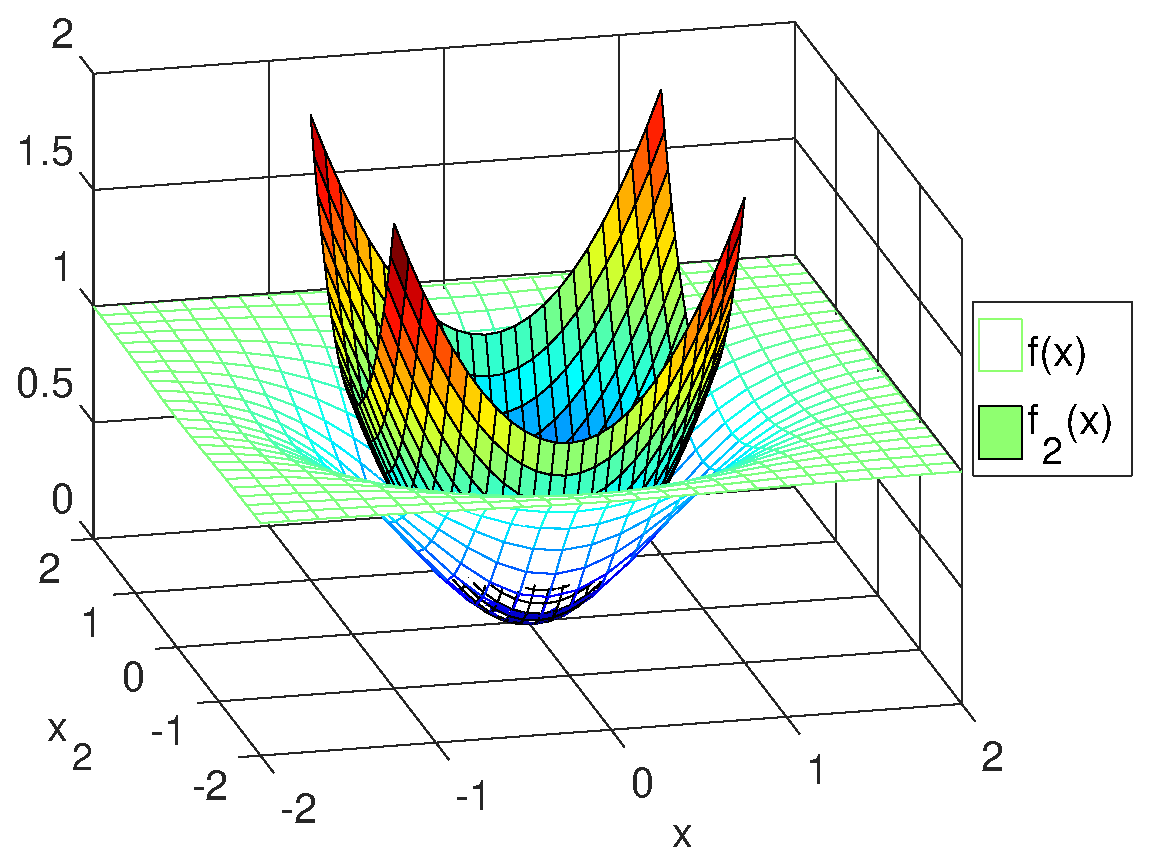
\includegraphics[width=0.5\textwidth]{chapters/funcoes/mcode/taylorR2R1/taylorf.eps}
  \caption{Aproximação $f_2(\VECTOR{x})$ da função $f(\VECTOR{x})$.}
    \label{fig:taylorf}
\end{figure}
 
%%%%%%%%%%%%%%%%%%%%%%%%%%%%%%%%%%%%%%%%%%%%%%%%%%%%%%%%%%%%%%%%%%%%%%%%%%%%%%%%%%%%%%%
\index{Serie de Taylor!$\VECTOR{f}:\mathbb{R}^{N}\rightarrow \mathbb{R}^{M}$}
\begin{proposition}[Serie de Taylor de $\VECTOR{f}(\VECTOR{x})$]\label{prop:taylorf}
Dada uma função  $\VECTOR{f}:\mathbb{R}^{N}\rightarrow \mathbb{R}^{M}$, 
sendo $\VECTOR{f}$ um vector coluna, com variável $\VECTOR{x} \in \mathbb{R}^{N}$, vetor coluna;
infinitamente diferenciável em $\VECTOR{a} \in \mathbb{R}^{N}$;
esta pode ser expressada mediante uma somatória, em serie de Taylor 
\cite[pp. 393]{levine1999control} \cite{Taylor} ao redor de $\VECTOR{a}$, como
mostra a Eq. (\ref{eq:taylorf1}),
\begin{equation}\label{eq:taylorf1}
\VECTOR{f}(\VECTOR{x}) =\VECTOR{f}(\VECTOR{a})
      ~+ \MATRIX{J}(\VECTOR{a}) (\VECTOR{x}-\VECTOR{a})
      ~+\cdots 
\end{equation}

Onde a matriz $\MATRIX{J}(\VECTOR{x})\equiv \frac{\partial \VECTOR{f}(\VECTOR{x})}{\partial \VECTOR{x}^{\transpose} }$,
também conhecido como matriz \hyperref[def:jacobian]{Jacobiana} de $\VECTOR{f}(\VECTOR{x})$.
\end{proposition}
